\documentclass[unicode,11pt,a4paper,oneside,numbers=endperiod,openany]{scrartcl}

\usepackage{assignment}
\usepackage{textcomp}
\hyphenation{PageRank}
\hyphenation{PageRanks}

\usepackage{listings}
\usepackage{color} %red, green, blue, yellow, cyan, magenta, black, white
\definecolor{mygreen}{RGB}{28,172,0} % color values Red, Green, Blue
\definecolor{mylilas}{RGB}{170,55,241}

\usepackage{graphicx}
\usepackage{caption}
\usepackage{subcaption}

\begin{document}

\lstset{language=Matlab,%
    %basicstyle=\color{red},
    basicstyle=\ttfamily\tiny,
    breaklines=true,%
    morekeywords={matlab2tikz},
    keywordstyle=\color{blue},%
    morekeywords=[2]{1}, keywordstyle=[2]{\color{black}},
    identifierstyle=\color{black},%
    stringstyle=\color{mylilas},
    commentstyle=\color{mygreen},%
    showstringspaces=false,%without this there will be a symbol in the places where there is a space
    numbers=left,%
    numberstyle={\tiny \color{black}},% size of the numbers
    numbersep=9pt, % this defines how far the numbers are from the text
    emph=[1]{for,end,break},emphstyle=[1]\color{red}, %some words to emphasise
    %emph=[2]{word1,word2}, emphstyle=[2]{style},    
}

\setassignment
\serieheader{
Software Atelier: Differential Equations}{Academic Year 2016/2017}{Instructor: Dr. Drosos Kourounis}{TA: Hardik Kothari}{Assignment 4 - FEM Solution of Poisson's equation in 3D}{}
\newline

\begin{center}
\begin{tabular}{rc}
Name: Juraj Kardos   & \rule{5cm}{0.0pt} \\
Discussed with: & \rule{5cm}{0.0pt} 
\end{tabular}
\end{center}



\section{The Problem}
We seek the discrete solution of Poisson's equation
\begin{align}
    -\nabla^2 u(x,y,z) &= f(x,y,z),\ (x,y,z) \in \Omega \\
    \frac{\partial u}{\partial n} &= 0, \quad y=1, z=1, \\
    u(x,y,z) &= u_0(x,y,z), \quad \text{otherwise}.
\end{align}
We assume unit cube domain $\Omega = [0,1]^3$ and use quadrilateral $N_x \times N_y \times N_z$ grid of trilinear hexahedron elements.

We want the exact solution of the PDE to be 
\begin{equation}
u_0(x,y) = xe^{-(y-1)^2(z-1)^2}.
\end{equation}

so we can compute $f(x,y)$ as following:
\begin{lstlisting}
syms x;
syms y;
syms z;
u = @(x,y,z) x * exp(- (y-1)^2 * (z-1)^2 );

u_xx = diff(u,x,2);
u_yy = diff(u,y,2);
u_zz = diff(u,z,2);

f = -(u_xx + u_yy + u_zz);

\end{lstlisting}

\section{FEM Solution}

\subsection{Mesh Generation}

The solution starts with generation of the mesh that approximates our domain. We assume unit square with non-overlapping elements. The domain is discretized by $N_x$ by $N_y$ by $N_z$ grid of nodes. The elements are defined by enumerating their vertices, we follow convention when enumerating the corners of the hexahedra element using VTK convention for element of type \texttt{VTK\_HEXAHEDRON}. For example, the bottom face of a single element would look like following:


\begin{lstlisting}
elements(id_elem,:) = [e, e+1, e+N_x+1, e+N_x,... ]
\end{lstlisting}

\subsection{Assembly of Discrete Operators}

Next step in FEM is assembly of discrete operators, namely mass matrix $M$, laplacian matrix $K$ and discretized RHS $b$. The idea of the assembly is to construct the local versions of the matrices and insert them into the global structure. 

\subsubsection{Mass Matrix}

Trilinear hexahedral element is defined by the following nodal functions:
\begin{align}
    N_1 &= \frac{1}{8} (1-\xi)(1-\eta)(1-\zeta), \\
    N_2 &= \frac{1}{8} (1+\xi)(1-\eta)(1-\zeta), \\
    N_3 &= \frac{1}{8} (1+\xi)(1+\eta)(1-\zeta), \\
    N_4 &= \frac{1}{8} (1-\xi)(1+\eta)(1-\zeta), \\
    N_5 &= \frac{1}{8} (1-\xi)(1-\eta)(1+\zeta), \\
    N_6 &= \frac{1}{8} (1+\xi)(1-\eta)(1+\zeta), \\
    N_7 &= \frac{1}{8} (1+\xi)(1+\eta)(1+\zeta), \\
    N_8 &= \frac{1}{8} (1-\xi)(1+\eta)(1+\zeta).
\end{align}
In order to compute integral over the domain of the element, we first project the hexahedral element $E$ wit coordinates  $(x_i,y_i,z_i), i \in [0,\ldots, 7]$ into reference element $E_0$ with coordinates $(\xi,\eta,\zeta)$in rage $[-1,1]$. The mapping is
\begin{align}
    x &= x_i + \frac{dx}{2} (\xi+1), \\
    y &= y_i + \frac{dy}{2} (\eta+1), \\
    z &= z_i + \frac{dz}{2} (\zeta+1).
\end{align}
For example, for reference coordinates of node $(\xi,\eta,\zeta)=(-1,-1,-1)$ we get coordinates of the node $(x_0,y_0,z_0)$ and for $(\xi,\eta,\zeta)=(1,-1,-1)$ we get node $(x_0+dx=x_1,y_0,z_0)$.

We define Jacobian of this transformation with respect to the reference coordinate frame $(\xi,\eta,\zeta)$, we get
\begin{equation}
    J = \begin{pmatrix}
    \frac{\partial x}{\partial \xi} &  \frac{\partial y}{\partial \xi} & \frac{\partial z}{\partial \xi} \\
    \frac{\partial x}{\partial \eta} &  \frac{\partial y}{\partial \eta} & \frac{\partial z}{\partial \eta} \\
    \frac{\partial x}{\partial \zeta} &  \frac{\partial y}{\partial \zeta} & \frac{\partial z}{\partial \zeta}
    \end{pmatrix} = 
    \begin{pmatrix}
     \frac {dx}{2} & 0 & 0 \\
     0 & \frac {dy}{2} & 0 \\
     0 & 0 & \frac {dz}{2}
    \end{pmatrix}.
\end{equation}

Computing integral over the reference integral is much easier, but we need to consider the transformation we did. This gives us 
\begin{align}
    m_{i,j} &= \int_{E} N_i(x,y,z) N_j(x,y,z) dE \\
    m_{i,j} &= \int_{E_0} J^{-1} N_i(x,y,z) J^{-1} N_j(x,y,z) |J| dE_0 \\
    m_{i,j} &= \int_{-1}^1 \int_{-1}^1 \int_{-1}^1 J^{-1} N_i(\xi,\eta,\zeta) J^{-1} N_j(\xi,\eta,\zeta) |J| d\xi d\eta d\zeta \\
    m_{i,j} &\approx \sum_{k_1=1}^n \sum_{k_2=1}^n \sum_{k_3=1}^n h_1 h_2 h_3 J^{-1}_{k1,k2,k3} N_i(\xi_{k1},\eta_{k2},\zeta_{k3}) J^{-1}_{k1,k2,k3} N_j(\xi_{k1},\eta_{k2},\zeta_{k3}) |J_{k1,k2,k3}|
\end{align}

The code implementing this is as following:
\begin{lstlisting}[caption=Local assembly of mass matrix]
xi = sym('xi', 'real');
eta = sym('eta', 'real');
zeta = sym('zeta', 'real');

dx = sym('dx', 'real');
dy = sym('dy', 'real');
dz = sym('dz', 'real');

%jacobian of the transformation
J(1,1) = 0.5*dx;
J(2,2) = 0.5*dy;
J(3,3) = 0.5*dz;

%nodal functions
c=[-1 -1 -1; 1 -1 -1; 1 1 -1; -1 1 -1; -1 -1 1; 1 -1 1; 1 1 1; -1 1 1];
for i=1:8
    N(i) = 1/8*( 1+c(i,1)*xi )*( 1+c(i,2)*eta )*( 1+c(i,3)*zeta );
end

%gaussian quadrature
F = det(J) * N' * N;
M = int(int(int(F, 'xi', -1, 1), 'eta', -1, 1), 'zeta', -1, 1);
\end{lstlisting}

\subsubsection{Laplacian matrix}

In a similar manner we construct the local Laplacian matrix. The integral over the element becomes
\begin{align}
    k_{ij} &= \int_{E} \nabla N_i (x,y,z) \nabla N_j(x,y,z) dE \\
    k_{ij} &= \int_{E_0} J^{-1} \nabla N_i (\xi, \eta, \zeta) J^{-1} \nabla N_j(\xi, \eta, \zeta) |J| dE_0 \\
    k_{ij} &= \int_{-1}^1 \int_{-1}^1 \int_{-1}^1 J^{-1} \nabla N_i (\xi, \eta, \zeta) J^{-1} \nabla N_j(\xi, \eta, \zeta) |J| d\xi d\eta d\zeta \\
    k_{ij} &\approx \sum_{k1=1}^n \sum_{k2=1}^n \int_{k3=1}^n h_1 h_2 h_3 J^{-1}_{k1,k2,k3} \nabla N_i (\xi_{k1}, \eta_{k2}, \zeta_{k3}) J^{-1}_{k1,k2,k3} \nabla N_j(\xi_{k1}, \eta_{k2}, \zeta_{k3}) |J_{k1,k2,k3}| d\xi d\eta d\zeta
\end{align}

\begin{lstlisting}[caption=Local assembly of Laplatian matrix]
xi = sym('xi', 'real');
eta = sym('eta', 'real');
zeta = sym('zeta', 'real');

dx = sym('dx', 'real');
dy = sym('dy', 'real');
dz = sym('dz', 'real');

%jacobain of the transformation
J(1,1) = 0.5*dx;
J(2,2) = 0.5*dy;
J(3,3) = 0.5*dz;

%nodal functions
c=[-1 -1 -1; 1 -1 -1; 1 1 -1; -1 1 -1; -1 -1 1; 1 -1 1; 1 1 1; -1 1 1];
for i=1:8
    N(i) = 1/8*( 1+c(i,1)*xi )*( 1+c(i,2)*eta )*( 1+c(i,3)*zeta );
end

%gradient of nodal funcitons
Nx = diff(N, 'xi');
Ny = diff(N, 'eta');
Nz = diff(N, 'zeta');

%gaussian quadrature
dN = [Nx; Ny; Nz];
Jd = inv(J) * dN;
F = det(J)*Jd'*Jd;
I = int(int(int(F, 'xi', -1, 1), 'eta', -1, 1), 'zeta', -1, 1);
\end{lstlisting}



After forming the local mass and Laplacian matrix for each element, we need to insert these into the global matrices $M$ and $K$. We do not insert elements one by one but we keep track of local indices and corresponding global indices in format of Matlab sparse matrix and we create matrix after all of the indices are available.

\subsection{Boundary Conditions}
We need to modify the equations for the points that lie on the boundary of our domain. The Dirichlet boundary specifies exact value of the target profile, that is $u(x,y,z) = u_0(x,y,z)$ for every $(x,y) \in \partial\Omega$ except for $y=1,z=1$ where Neumann BC apply.

Neumann BC specify not the target profile of the domain, but the rate of the change of the domain. Basically, a Dirichlet BC means imposing the value for the temperature (or some other physical quantity) in one edge of the dimensional domain (a metal bar, for example), i.e. fixing the value for the temperature for the solution at that edge while Newmann BC mean to impose the flux of heat through that edge. If Newmann BC is set to zero (homogeneous BC) it means that the edge of the bar is isolated and no flux of heat enters or outputs the bar.

To verify that NBC hold we should check that the following relations are satisfied:
\begin{align}
    \frac{\partial u}{\partial n_{y=1}} &= 0 \\
    \frac{\partial u}{\partial n_{z=1}} &= 0
\end{align}
The unit normal $n$ at the faces of the cube where $y=1$ and $z=1$ is simply $y$ and $z$ respectively, so we need to do partial derivatives. In this case the BC are homogeneous, that is they are equal to $0$ so they do not influence the solution. But if this was not the case we would have to adjust the RHS term at appropriate positions (after deriving the weak formulation Neumann BC show up on RHS).

\begin{lstlisting}
% impose boundary conditions for Dirichlet boundaries
I = find(mesh.PointMarkersDiri);

%adjust K
K(I,:) = 0;
for i = 1:length(I);
  K(I(i),I(i)) = 1.0;
end

%adjust RHS
X = mesh.Points(I,1);
Y = mesh.Points(I,2);
Z = mesh.Points(I,3);
b(I) = u0(X,Y,Z);
\end{lstlisting}

\subsection{Solution}
Having the system ready at hand, we need to solve it. In vector $u$ we will have approximate solution to our problem.
\begin{lstlisting}
% solve
u = K\b;

% visualize solution
writeMeshToVTKFile(mesh, x, 'solution')
\end{lstlisting}


\begin{figure}
    \centering
    \begin{subfigure}[b]{0.48\textwidth}
        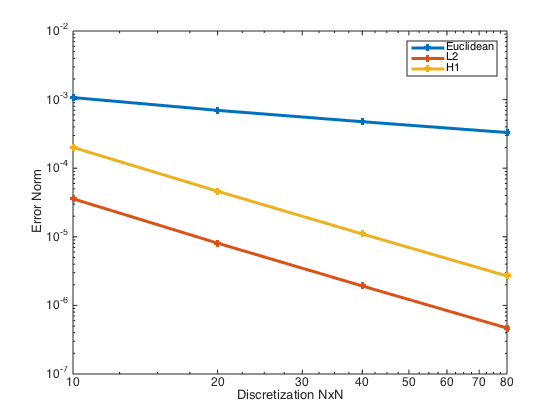
\includegraphics[width=\textwidth]{../FEMerror}
        \caption{Error norms}
        \label{fig:gull}
    \end{subfigure}
    ~ %add desired spacing between images, e. g. ~, \quad, \qquad, \hfill etc. 
      %(or a blank line to force the subfigure onto a new line)
    \begin{subfigure}[b]{0.48\textwidth}
        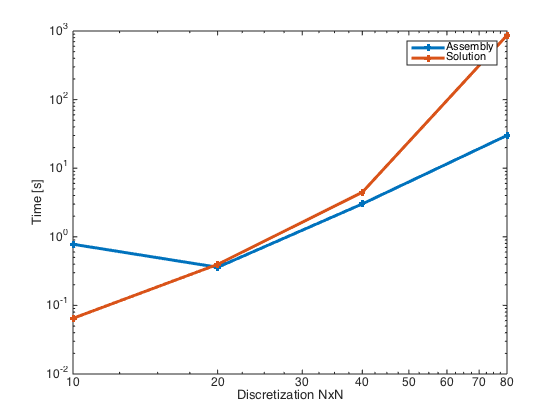
\includegraphics[width=\textwidth]{../FEMtime}
        \caption{Solution time}
        \label{fig:tiger}
    \end{subfigure}
    \caption{Discretizations \texttt{10,20,40,80}}\label{fig:animals}
\end{figure}

\subsection{Visualization of the Solution}
\begin{figure}
    \centering
    \begin{subfigure}[b]{0.45\textwidth}
        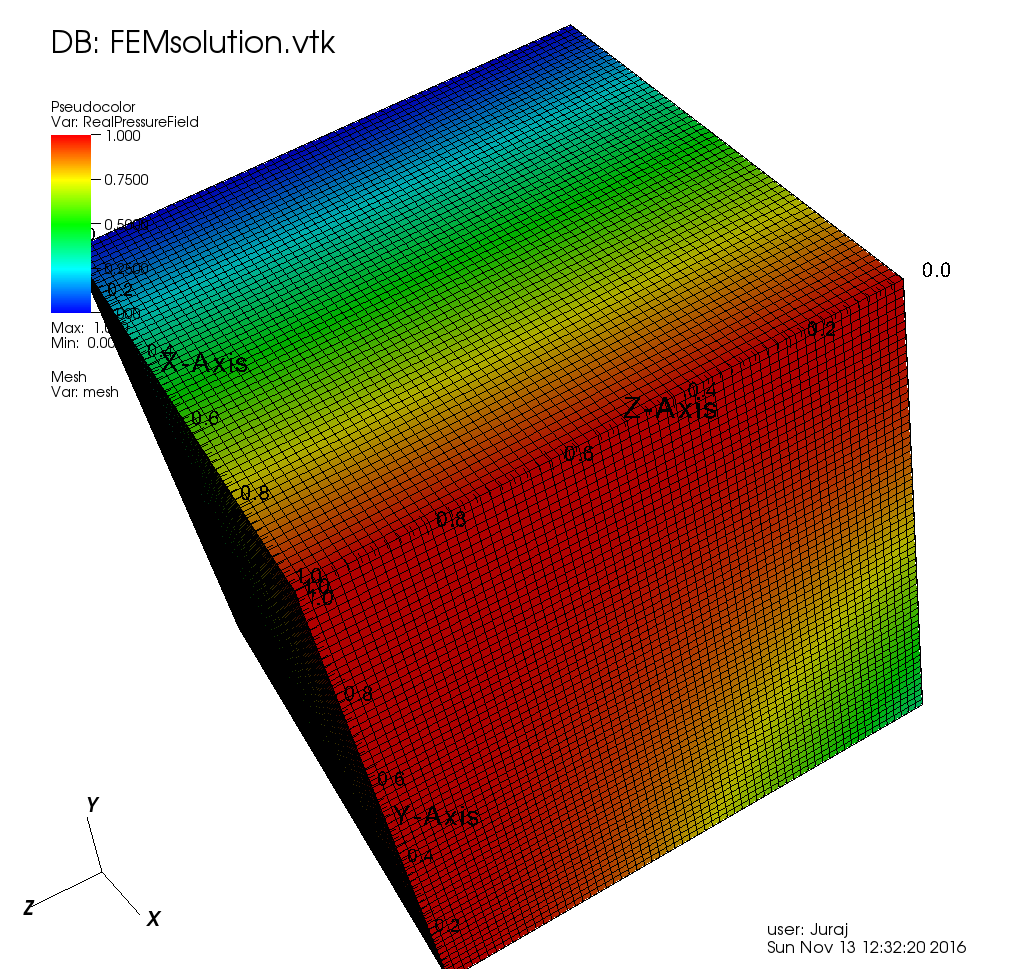
\includegraphics[width=\textwidth]{../FEMsolution}
        \caption{FEM solution for $N=60$}
        \label{fig:gull}
    \end{subfigure}
    ~ %add desired spacing between images, e. g. ~, \quad, \qquad, \hfill etc. 
      %(or a blank line to force the subfigure onto a new line)
    \begin{subfigure}[b]{0.45\textwidth}
        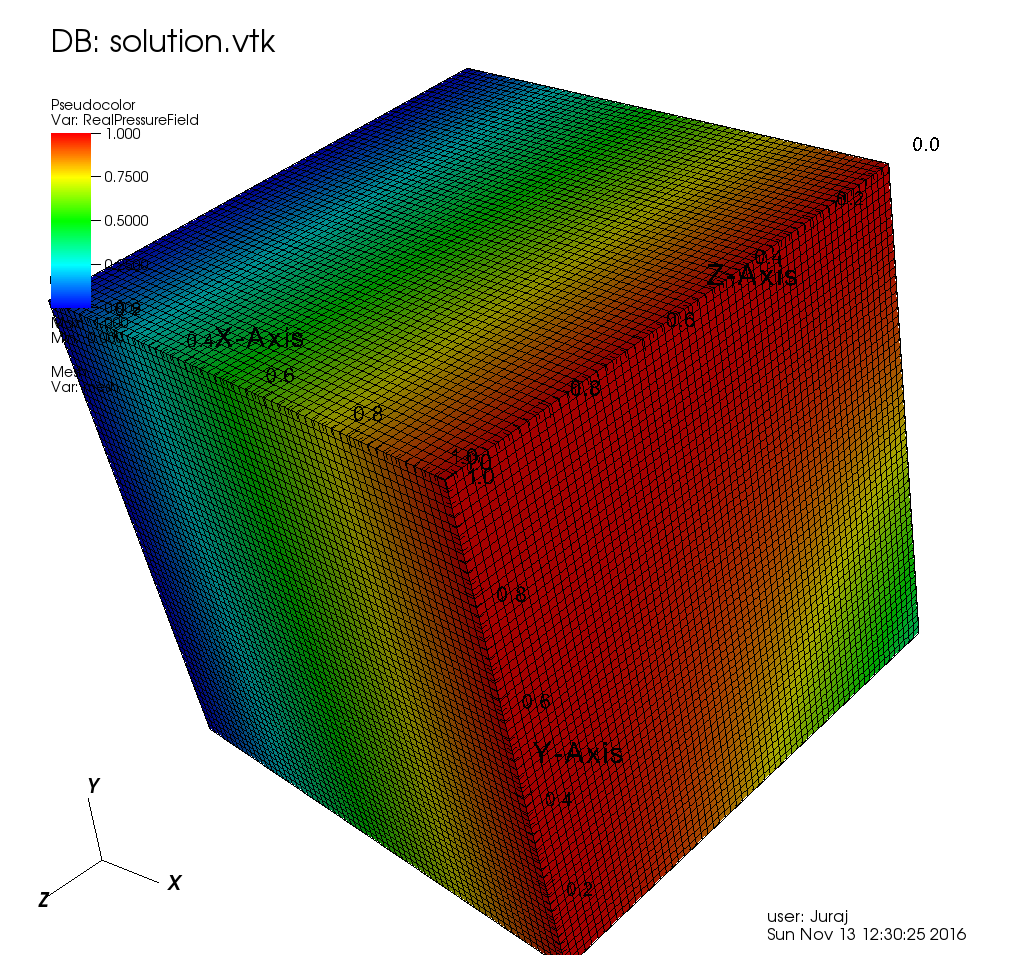
\includegraphics[width=\textwidth]{../solution}
        \caption{Exact solution}
        \label{fig:tiger}
    \end{subfigure}
    \caption{Solution of $u$}\label{fig:animals}
\end{figure}

\end{document}
